\documentclass[titlepage]{article}
\usepackage[utf8]{inputenc}
\usepackage{geometry}
\geometry{a4paper, margin=1in}
%\usepackage[draft]{graphicx} %uncomment this for faster compiles.
\usepackage{graphicx}  %uncomment this for pictures to load in.
\usepackage{float}
\usepackage{subcaption}
\usepackage{listings}
\usepackage{caption}
\usepackage[table]{xcolor} % Enable coloring of table cells
\usepackage{booktabs} % For formal tables
\usepackage{array}
\definecolor{lightgray}{gray}{0.9}

\begin{document}


\title{Software Design Document\\ \textbf{Insight Glass}}
\author{Aser Osama - 202101266 \\ Aya Sherif - 202100642 \\ Gehan Sherif - 201902069 \\ Omar Ayman 202100443 }
\date{Version 1.0 \\\ \today}


\maketitle
 \tableofcontents


\newpage

\section{Project Overview}
\subsection{Project idea}
Our project's main goal is to help professionals from different disciplines start their careers at companies where 
they can thrive. This will be achieved through radical transparency of the companies, breaking down all barriers 
and problems in the Egyptian job markets that lead to discrimination, pay gaps, and toxic work environments.

\subsection{Vision}
The vision is to transform the Egyptian job market by empowering individuals to make informed decisions about their 
career path. The project aims to address common issues of job seekers struggling to identify suitable employment 
opportunities and being locked into unfavorable work environments due to contractual obligations. By providing 
comprehensive insight into the company and facilitating transparent communication between job seekers and 
employers, the project seeks to create a dynamic ecosystem that fosters mutual growth, and they are satisfied 

\subsection{Competitive Analysis}
In Egypt's job market, traditional methods of hiring still dominate, with a reliance on personal connections and 
in-person applications. However, the emergence of online platforms has introduced new avenues for job 
seekers. Two prominent competitors in this space are Glassdoor.

\subsubsection*{Glassdoor}
Glassdoor, our main competitor, is a well-established platform known for providing company reviews, salary information, and job 
listings. While it offers valuable insights into company cultures and employee experiences globally, its 
adaptation to the Egyptian context might be limited. Glassdoor primarily relies on user-generated content, 
which may vary in quantity and quality, especially for companies with a smaller presence in Egypt. 
Additionally, the platform's focus on larger corporations might overlook opportunities within smaller or niche 
companies in the Egyptian job market.

\newpage

\section{System Technical Overview}
\subsection{System Architecture}
We will use a simple, reliable, yet scalable architecture. We will use a Frontend and API connecting to a 
backend model. It is a simple model, however, it will be comfortably scalable using Kubernetes, Azure, or any 
other load balancers as we expand to have more people using our service. We will use virtualization in
expandability and have spare servers be there in case of breakdowns to minimize downtime. 

\begin{figure}[H]
    \centering
    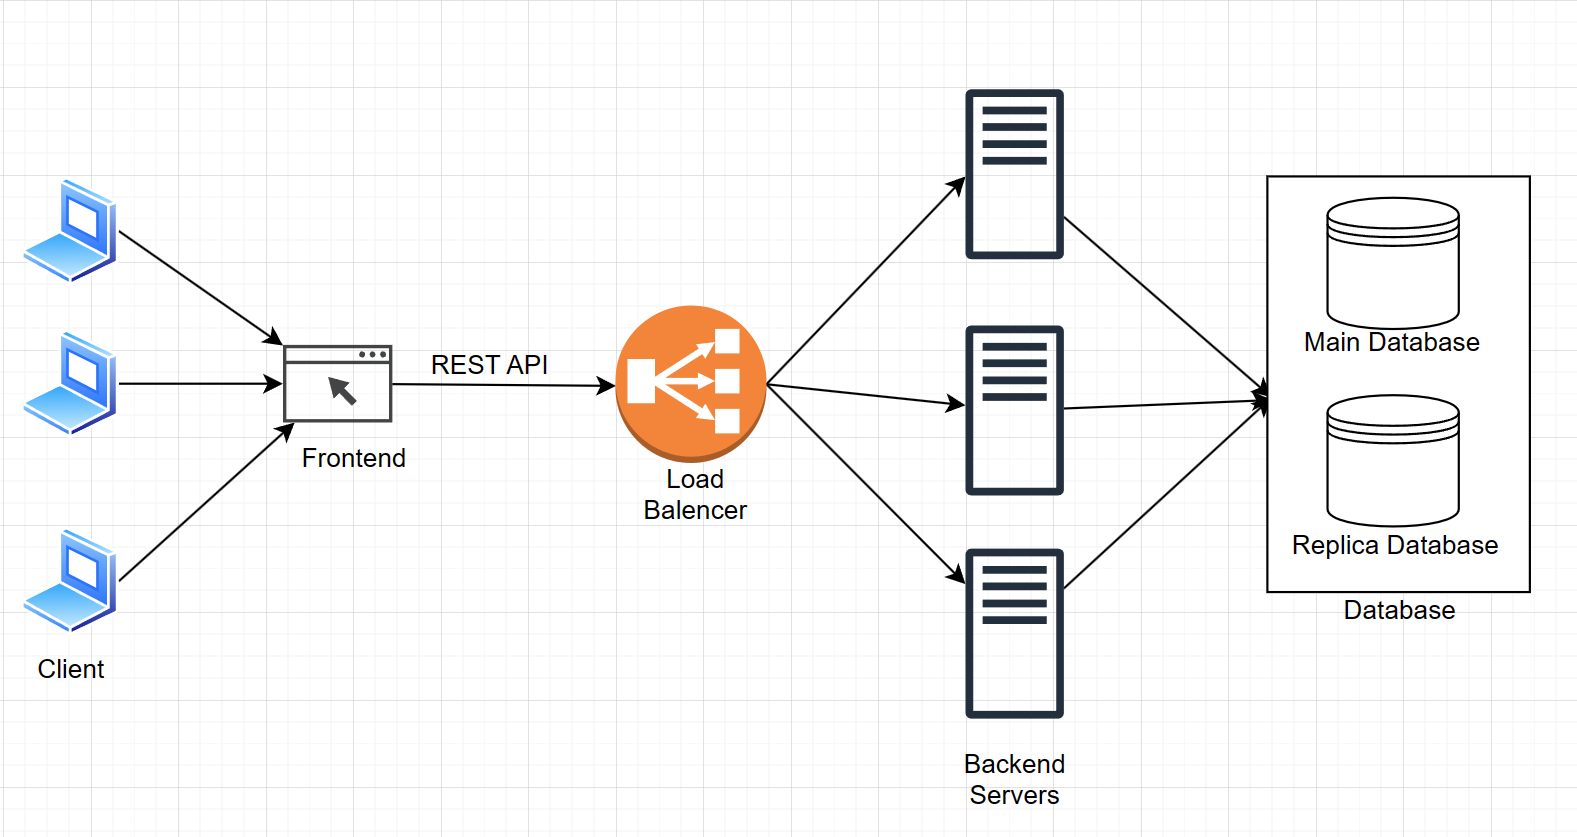
\includegraphics[width=0.8\textwidth]{Images/ArchOverview.png}
    \caption{System Architecture Overview}
\end{figure}

\subsection{Used Technologies}
\begin{itemize}
    \item \textbf{Frontend:} React.js for building a responsive and dynamic user interface
    \item \textbf{Backend:} ASP.NET Web API in .NET 8 for server-side logic, providing a reliable and efficient foundation.
    \item \textbf{Database:} MySQL/MariaDB for storing user data, reviews, and job listings, chosen for its flexibility with 
    schema design and easy to find support. Interaction with the database will be through the Entity Framework 
    Core ORM
    \item \textbf{Authentication:} Identity framework with cookie-based authentication will be used.
\end{itemize}

\newpage

\section{Biggest Challenges and Mitigations}
\subsection{Challenges}
Egypt is currently very behind in terms of modernizing the hiring process, therefore it would be incredibly 
difficult to try and convince companies and people to change their old ways. Adoption of the application will 
also be difficult due to the reason we would most likely function as a startup which is also not looked to highly 
of in Egypt. Aside from initial adoption of the application, building a community of verified employees to 
provide us with reviews and insight might be also difficult as people tend to not be as open with salaries or job 
experience here. We will be challenging a lot of old stereotypes and set in stone rules of the workplace with our 
application. A more technical issue we might face are fake reviews. Finally, the legalities of sharing job reviews 
and such are not too certain in Egypt so it could be risky if not dealt with correctly.

\subsection{Solutions}
The technical issue of fake reviews could be easily solved by adding multiple human verification stages to our 
website as well as requiring identification and proof of employment to be able to post reviews that would affect 
the overall company rating while also keeping a section for unverified reviews. As for the adoption issues,
however, we could attempt to gain the user’s trust by getting affiliation with trusted companies or businesses 
figures. However, it is most likely that the issue would simple be resolved with time and we have no real choice 
to kickstart our popularity. Finally, for the legalities, we could employee a part time or on demand legal team to 
help us sort it out.

\section{Feasibility Matrix}

%colorless table:
% \begin{table}[h]
% \centering
% \caption{Feasibility Assessment}
% \label{tab:feasibility_assessment}
% \begin{tabular}{@{}lp{5cm}ccc@{}}
% \toprule
% Criteria             & Description                                                                                        & Score & Weight & Total Score \\ \midrule
% Technical Feasibility & The project's technical requirements include platform development and data gathering processes.     & 4     & 25     & 100        \\
% Economic Feasibility  & The financial viability of the project, including initial investment, operating costs, and revenue generation. & 3     & 20     & 60         \\
% Legal Feasibility     & Compliance with legal regulations and potential risks related to data privacy, intellectual property, etc.        & 4     & 20     & 80         \\
% Operational Feasibility & The project's practical implementation and operational processes, including user engagement and support.  & 5     & 35     & 175        \\ \bottomrule
% \end{tabular}
% \end{table}

\begin{table}[h]
    \centering
    \caption{Feasibility Assessment}
    \label{table:feasibility}
    \begin{tabular}{>{\raggedright}m{3.5cm} >{\raggedright\arraybackslash}m{5.5cm} c c c}
    \toprule
    \textbf{Criteria} & \textbf{Description} & \textbf{Score} & \textbf{Weight} & \textbf{Total Score} \\ 
    \midrule
    \rowcolor{lightgray} Technical Feasibility & The project's technical requirements include platform development and data gathering processes. & 4 & 25 & 100 \\
    Economic Feasibility & The financial viability of the project, including initial investment, operating costs, and revenue generation. & 3 & 20 & 60 \\
    \rowcolor{lightgray} Legal Feasibility & Compliance with legal regulations and potential risks related to data privacy, intellectual property, etc. & 4 & 20 & 80 \\
    Operational Feasibility & The project's practical implementation and operational processes, including user engagement and support. & 5 & 35 & 175 \\
    \bottomrule
    \end{tabular}
    \end{table}

\newpage
\section{GUI for functional requirements}
\subsection{User Interfaces}
Below are pages that shows the main flow and functionality of Insight Glass
\begin{enumerate}
    \item First view of the home page
    \begin{figure}[H]
        \centering
        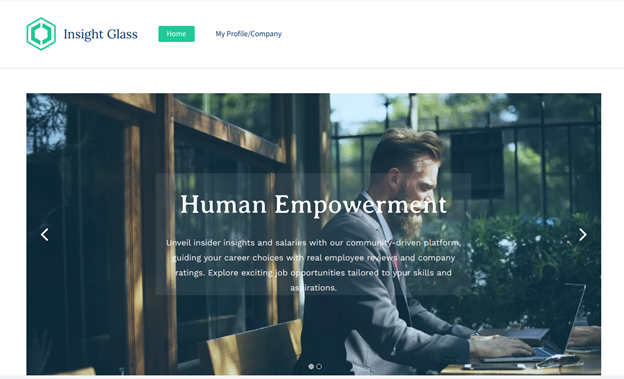
\includegraphics[width=0.75\textwidth]{Images/Home_page_first_view.png}
        \caption{First view of the home page (1 out of 2)}
    \end{figure}
    \begin{figure}[H]
        \centering
        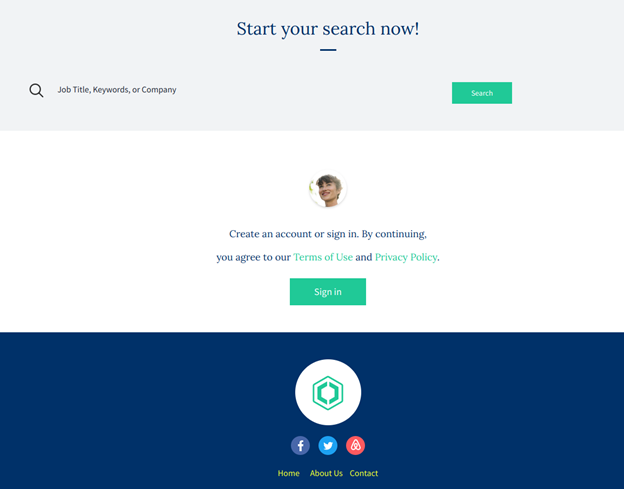
\includegraphics[width=0.75\textwidth]{Images/Home_page_first_view_2.png}
        \caption{First view of the home page (2 out of 2)}
    \end{figure}
    \newpage
    \item Second view of the home page
    \begin{figure}[H]
        \centering
        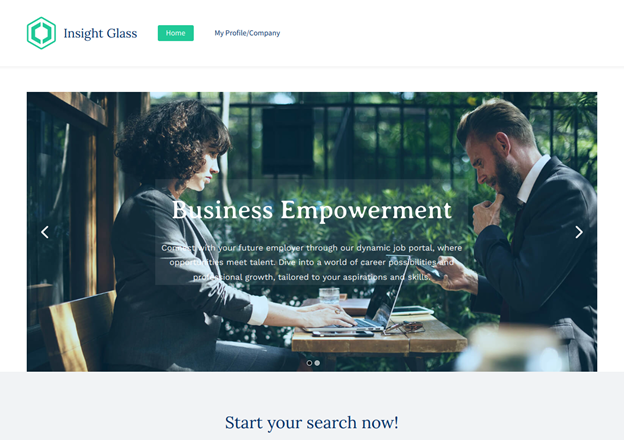
\includegraphics[width=0.75\textwidth]{Images/Home_page_second_view.png}
        \caption{Second view of the home page}
    \end{figure}
    \begin{figure}[H]
        \centering
        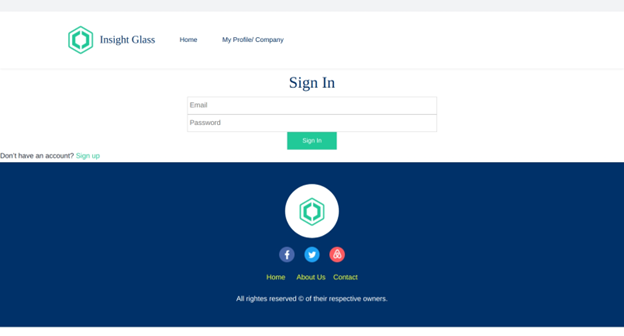
\includegraphics[width=0.75\textwidth]{Images/sign_in.png}
        \caption{Sign in page}
    \end{figure}
    \newpage
    \item Sign up page 
    \begin{figure}[H]
        \centering
        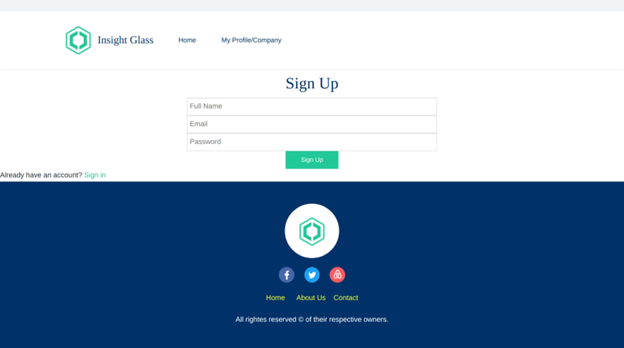
\includegraphics[width=0.75\textwidth]{Images/Sign up.png}
        \caption{Sign up page}
    \end{figure}
    \item User profile
    \begin{figure}[H]
        \centering
        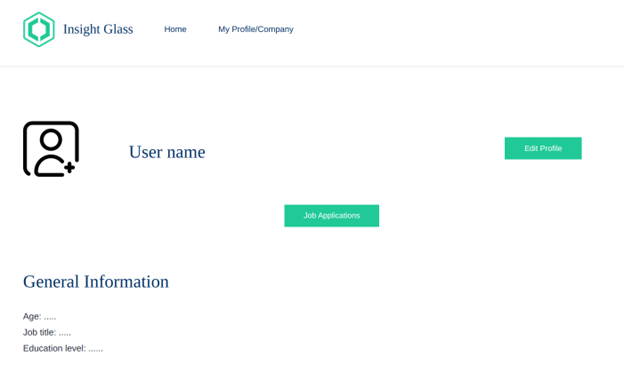
\includegraphics[width=0.75\textwidth]{Images/User_profile_1.png}
        \caption{User profile page (1 out of 2)}
    \end{figure}
    \begin{figure}[H]
        \centering
        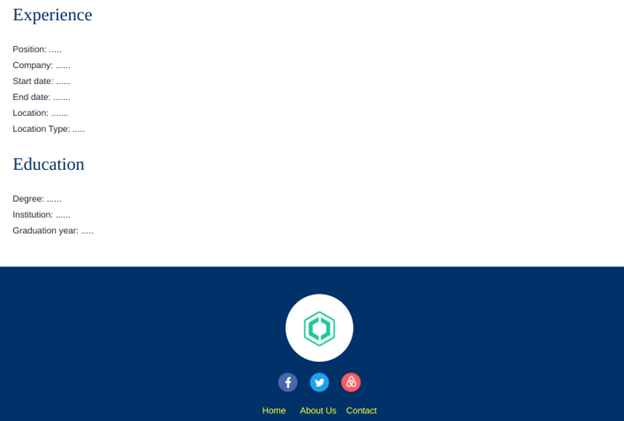
\includegraphics[width=0.75\textwidth]{Images/User_profile_2.png}
        \caption{User profile page (2 out of 2)}
    \end{figure}
    \item Company Profile
    \begin{figure}[H]
        \centering
        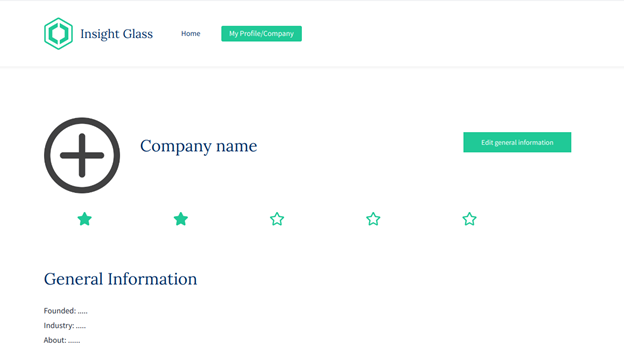
\includegraphics[width=0.75\textwidth]{Images/Company_profile_1.png}
        \caption{Company profile page (1 out of 2)}
    \end{figure}
    \begin{figure}[H]
        \centering
        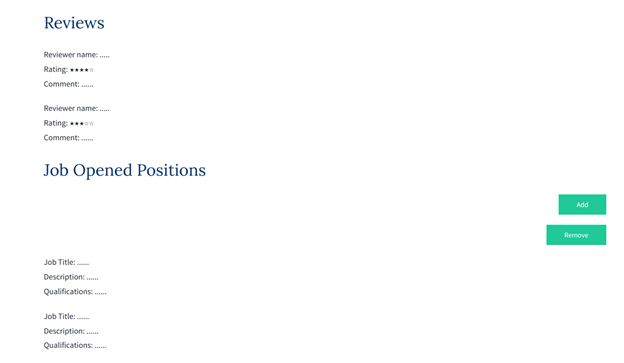
\includegraphics[width=0.75\textwidth]{Images/Company_profile_2.png}
        \caption{Company profile page (2 out of 2)}
    \end{figure}
    \item Search for a job page 
    \begin{figure}[H]
        \centering
        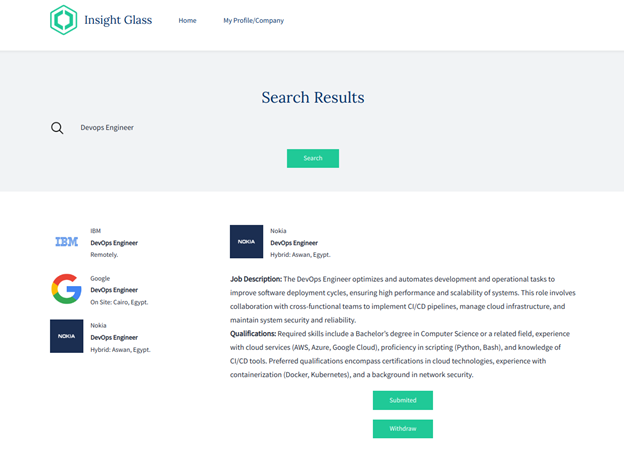
\includegraphics[width=0.75\textwidth]{Images/Search_for_job.png}
        \caption{Search for a job page}
    \end{figure}
    \newpage
    \item Search for a company page
    \begin{figure}[H]
        \centering
        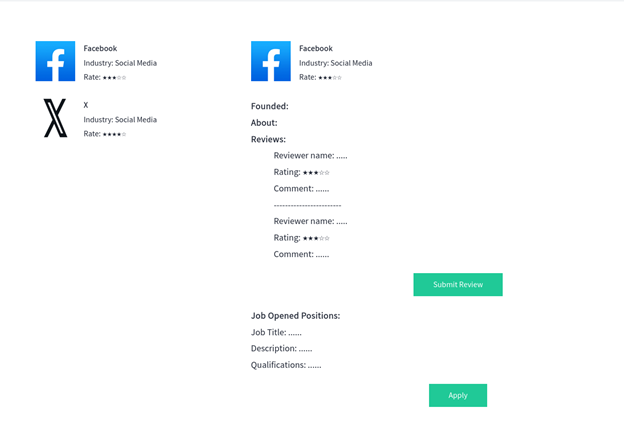
\includegraphics[width=0.75\textwidth]{Images/search_for_company.png}
        \caption{Search for a company page}
    \end{figure}
    \item Admin page
    \begin{figure}[H]
        \centering
        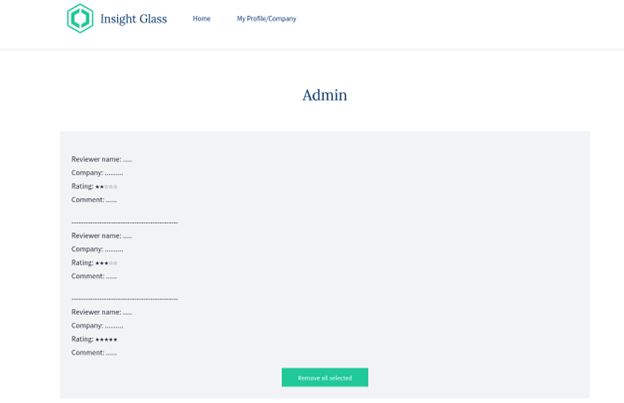
\includegraphics[width=0.75\textwidth]{Images/Admin_page.png}
        \caption{Admin page}
    \end{figure}
\end{enumerate}
\newpage
\section{System Design}
Below is the class diagram of the main objects in Insight Glass:
\begin{figure}[H]
    \centering
    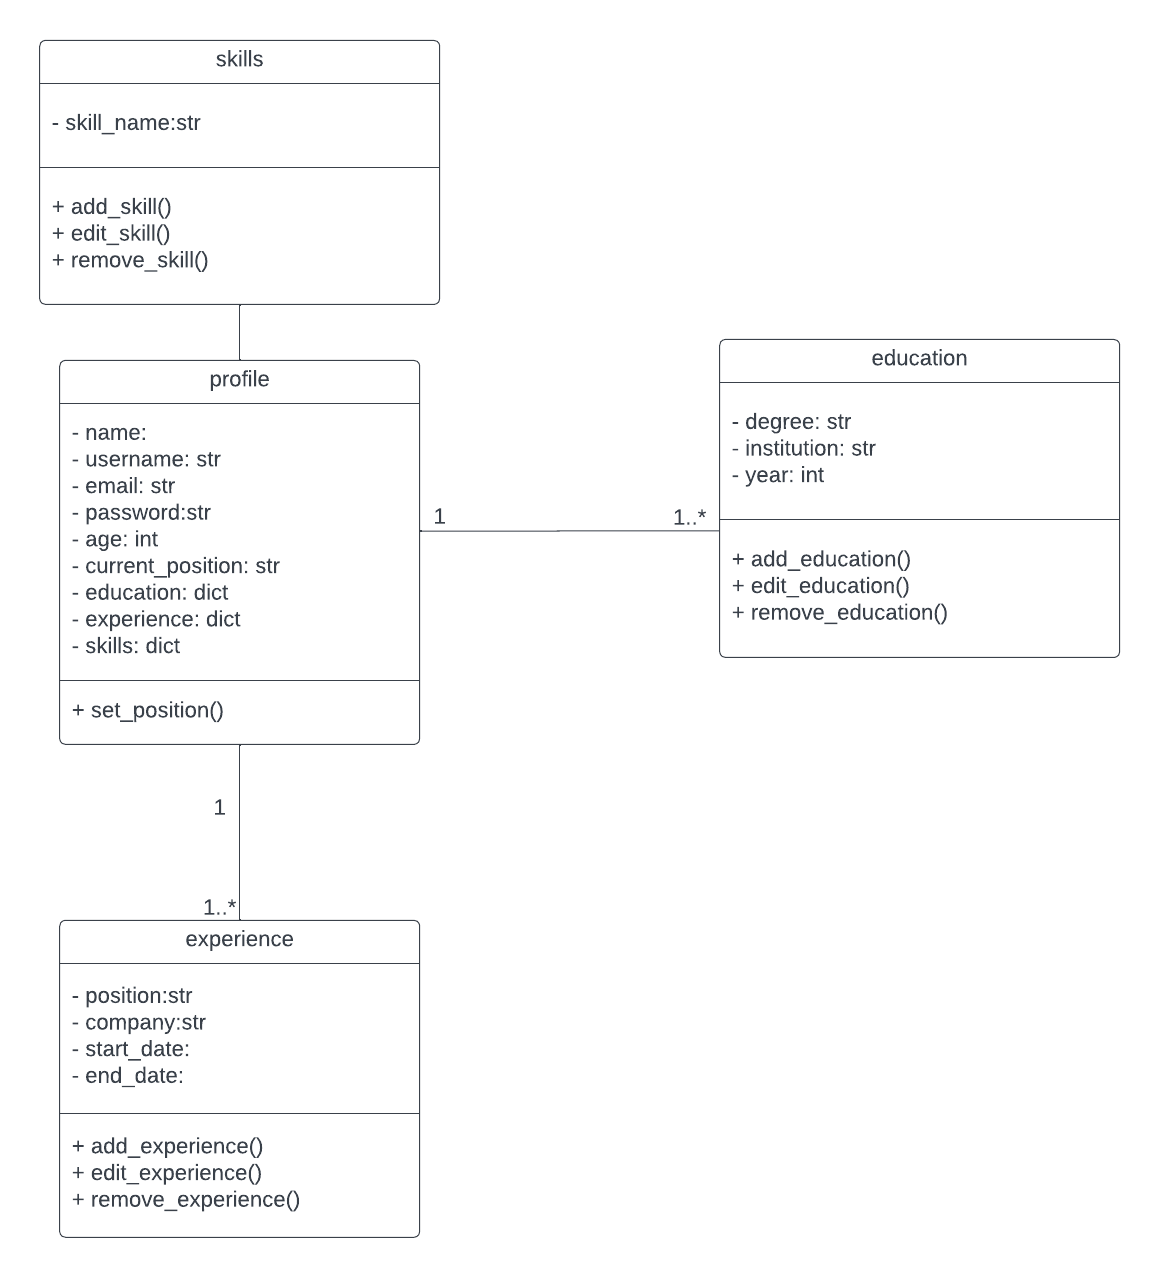
\includegraphics[width=1\textwidth]{Images/class_I.png}
    \caption{Classes of Insight Glass}
\end{figure}

\begin{figure}[H]
    \centering
    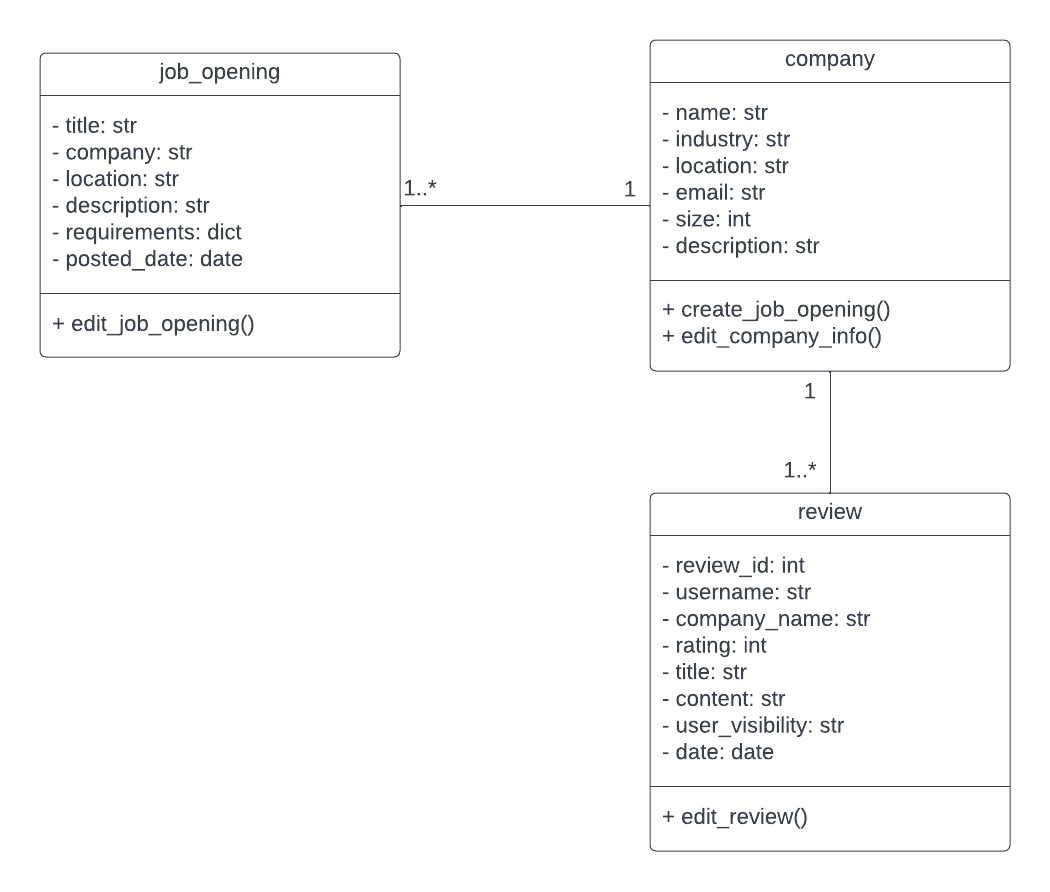
\includegraphics[width=0.75\textwidth]{Images/class_II.png}
    \caption{Classes of Insight Glass}
\end{figure}
\newpage
In the following use case diagram, we depict how a user can search for some company and sort their choices using Insight Glass functionalities.
\begin{figure}[H]
    \centering
    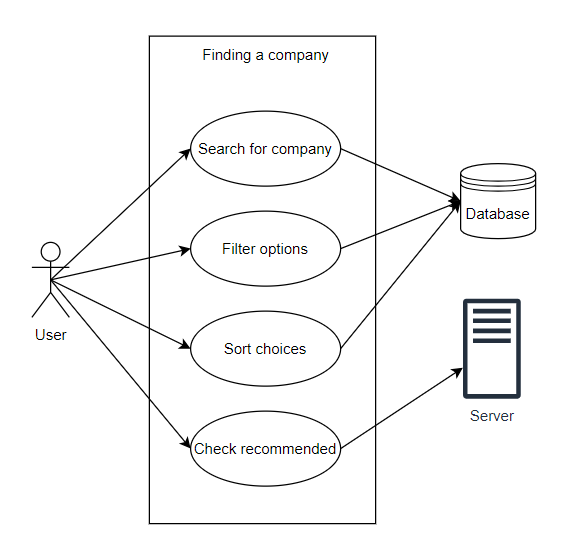
\includegraphics[width=0.75\textwidth]{Images/use_case.PNG}
    \caption{Use case diagram for finding a company}
\end{figure}
Another use case diagram shows how an employee can give a feedback for a certain company.
\begin{figure}[H]
    \centering
    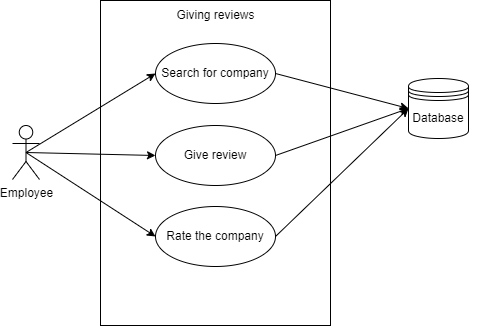
\includegraphics[width=0.75\textwidth]{Images/Reviews.png}
    \caption{Context diagram for Insight Glass}
\end{figure}
A third use case diagram shows how a job seeker can search for a job, shown below.
\begin{figure}[H]
    \centering
    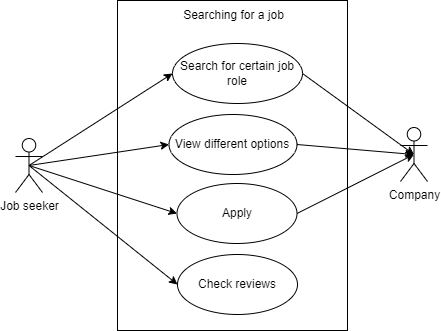
\includegraphics[width=0.75\textwidth]{Images/Searching.png}
    \caption{Context diagram for Insight Glass}
\end{figure}
The following is a context diagram that represents the relationship between
data and business processes visually.
\begin{figure}[H]
    \centering
    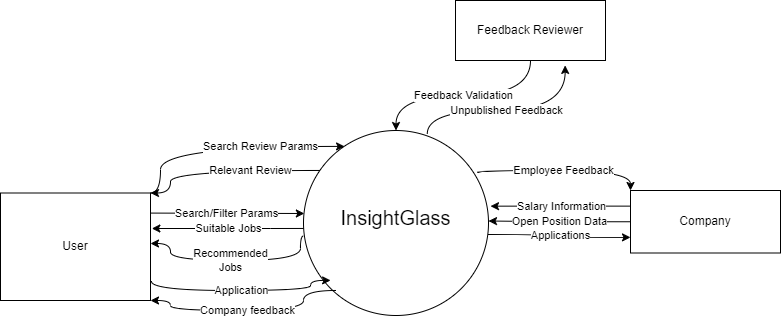
\includegraphics[width=0.9\textwidth]{Images/context_diagram.png}
    \caption{Context diagram for Insight Glass}
\end{figure}
The relations between different classes and packages of the system can be shown using a conceptual model as in the figure below.
\begin{figure}[H]
    \centering
    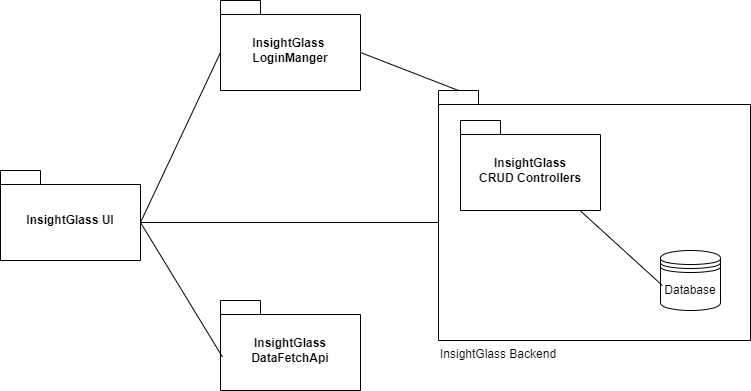
\includegraphics[width=0.75\textwidth]{Images/Conceptual.png}
    \caption{Conceptual model for Insight Glass}
\end{figure}
\section{Functional Requirements}
\subsection{User Registration and Authentication:}
\begin{itemize}
    \item Users can create an account by providing basic information such as email, username, and password.
    \item Users can authenticate their account through email verification or other methods to ensure security.
\end{itemize}
\subsection{Profile Management:}
\begin{itemize}
    \item Users can create and maintain a personal profile showcasing their skills, experience, and education.
    \item Users can edit and update their profile information, including work history, education, certifications, and skills.
    \item Users can upload and manage their resume, cover letters, and other relevant documents.
\end{itemize}

\subsection{Advanced Job Search Filters:}
\begin{itemize}
    \item Users can search for job openings by keyword, location, industry, or company.
    \item User can filter job listings based on criteria such as salary, job type, and experience level.
\end{itemize}

\subsection{Comprehensive Company Profiles:}
\begin{itemize}
    \item Users can request the inclusion of companies not listed on the platform, expanding the range of available job opportunities. For example, a CEO of a software company can create a profile for his company.
    \item Users can access detailed profiles of companies, providing comprehensive information about the organization.
    \item Users can view key details such as company size, revenue, headquarters location, and founding year.
    \item Users can view employee testimonials to gain insights into the workplace environment.
\end{itemize}

\subsection{Transparent Job Listings:}
\begin{itemize}
    \item Users can access job listings that provide detailed information about the position, including responsibilities, qualifications, and benefits.
    \item Users can access insights or reviews from current or former employees about the hiring company to gain context about the work environment.
    \item Users can track the status of their applications and receive updates or notifications about changes in the job listing, such as application deadlines or interview invitations.
\end{itemize}

\subsection{Career Advice:}
\begin{itemize}
    \item Users can access articles, tips, and resources related to career development, job searching, and workplace issues.
    \item Users can participate in forums or Q\&A sections to seek advice from experts and peers.
    \item Users can receive personalized career advice based on their interests, goals, and experience level,
\end{itemize}

\subsection{Interactive Discussion Forums:}
\begin{itemize}
    \item Users can join specialized chat channels or forums dedicated to some disciplines as software engineering to discuss different offers and job opportunities.
    \item Users can engage with industry experts or mentors through Q\&A sessions, AMA (Ask Me Anything) events, or one-on-one consultations.
\end{itemize}

\subsection{Direct Communication Channels:}
\begin{itemize}
    \item Users can directly message companies or hiring managers to inquire about job openings, company culture, and application processes.
    \item Job seekers can gather more information about potential employers before applying to a specific job opening.
\end{itemize}
\subsection{Salary Benchmarking Tools:}
\begin{itemize}
    \item Users should have access to comprehensive salary data for various job positions and industries, giving insights into average salaries, salary ranges, and compensation trends for specific roles and geographic locations.
    \item Users can compare their salary against peers with similar backgrounds, roles, and experience.
    \item Salary benchmarking tools offer visualizations such as charts, graphs, and reports to present salary data in an easily digestible format.
\end{itemize}

\subsection{Feedback and Ratings System:}
\begin{itemize}
    \item Users can provide feedback and ratings on their experiences with companies, including aspects such as company culture, work-life balance, management, and career growth opportunities. Reviews and ratings may be subject to verification processes to ensure their authenticity and reliability.
    \item Users can rate companies, job listings, and interview experiences on a standardized scale (e.g., star ratings or numerical scores).
    \item Users have the option to provide feedback anonymously, allowing them to share honest and candid opinions without fear of repercussions.
\end{itemize}
\subsection{Integration with Social Media Platforms:}
\begin{itemize}
    \item Users can easily share job listings, company profiles, and other relevant content from the platform to their social media accounts.
    \item Users have the option to link their platform profiles with their social media accounts, increasing their visibility and networking opportunities.
    \item Employers and recruiters can promote job openings and employer branding initiatives through their social media channels, reaching a broader audience of potential candidates.
\end{itemize}
\subsection{Interview Preparation Resources:}
Users can share and access interview experiences specific to the Egyptian job market, including insights on common interview questions, cultural expectations, and company-specific practices.
\begin{itemize}
    \item Users can access comprehensive guides and resources to prepare for various types of interviews, including behavioral interviews, technical interviews, case interviews, and competency-based interviews.
    \item Users can receive feedback on their resumes, cover letters, and portfolios from industry experts or career coaches.
\end{itemize}

\subsection{Analytics and Insights Dashboard:}
\begin{itemize}
    \item Administrators should have access to an analytics and insights dashboard to track user engagement, job market trends, and platform performance metrics. The dashboard shhould provide comprehensive data visualization and analysis tools for monitoring user activity, such as job searches, applications, and interactions.
\end{itemize}
\section{Non-Functional Requirements}
\subsection{Performance and Scalability}

The platform   should be highly responsive, with fast loading times and smooth navigation, ensuring a seamless user experience for job seekers and employers accessing the platform from various devices and locations across Egypt.
The system architecture should be scalable to accommodate growing user traffic and data volume, allowing the platform to handle increased user activity and maintain performance reliability during peak usage periods.
\subsection{Data Privacy and Security Compliance}

The platform should adhere to strict data privacy and security standards, ensuring the confidentiality, integrity, and availability of user data.
Compliance measures should align with Egyptian data protection regulations, such as the Data Protection Law, ensuring that user information is stored, processed, and transmitted securely to mitigate the risk of unauthorized access, data breaches, and privacy violations.
\appendix
\section{Appendix A: Glossary}
\section{Appendix B: Feasibility Study}
\section{Appendix C: Issue Log}

\end{document}
